\chapter{El Problema}


\section{Introducción}

En esta sección buscaremos dar una descripción mas detallada, tanto del problema a resolver, como así también de cada una de las soluciones adoptas durante el desarrollo del mismo. Sin embargo, queda fuera del alcance de
este documento los detalles de las técnicas utilizada(Reinforcement Learning y Deep Learning), pues consideramos que existen otros recursos donde explican detalladamente ambas. (ver Capitulo 7 - Bibliografía).
\\\\
Recordemos que el objetivo es desarrollar un agente inteligente, que a partir de un capital inicial, sea capaz de realizar compras y ventas de un activo dentro de un mercado financiero. El agente no poseerá ningún conocimiento previo acerca del funcionamiento del mercado, ni de la empresa sobre la que opera, ni ningun otro tipo de información. Solo conocerá el precio actual de la acción, y su evolución durante los días previos, junto un conjunto de indicadores bursátiles. 
\\
El agente va a interactuar con un simulador de un mercado bursátil, esta interacción se llevará a cabo siguiendo una serie de acciones, observaciones y recompensas.
Cada interacción será llevada a cabo en episodios que tendrán una duración de m días
\\

\begin{figure}[h!]
	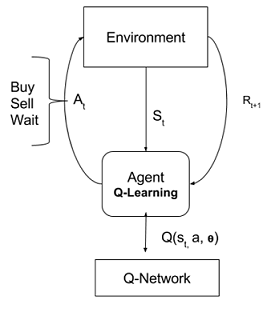
\includegraphics[scale=0.5]{imagenes/deepRLOverview.png}
	\caption{Reinforcement Learning Architecture Overview.}
\end{figure}


En cada instante t, el agente tendrá que seleccionar una acción $a_t$  de un conjunto válido de acciones A = {$a_1$, $a_2$, …, $a_n$}. La acción será pasada al entorno, el cual modificará su estado interno y como respuesta a esta interacción el agente recibirá una recompensa (reward R\textsubscript{t + 1}), la cual será calculado por el entorno. El entorno será estocástico, es decir, su comportamiento será no determinístico. Cada uno de los estados contendrá información relevante sobre el papel, como el precio, el volumen, y diferentes indicadores bursátiles, como medias móviles, medias móviles exponenciales, etc.

\section{Configuración de estados}

Ya sea de que se trate de un inversor experimentado o un agente inteligente, difícilmente sea posible tomar una decisión acertada sobre, la compra o venta de un activo, solamente mirando lo que sucede con el precio actual 
del activo, es necesario considerar una ventana de tiempo de tamaño n, para poder analizar la variación que ha tenido y así poder determinar la situación actual del activo, es decir, si se encuentra en una tendencia
alcista o bajista, si se encuentra realizando una corrección de precio o no, si se encuentra en sobre compra o sobre venta, etc. Una manera eficiente de ver esto, es a través, de un gráfico de vela, donde cada vela, representa un periodo, el cual puede ser, un año, una semana, o un mes.

\begin{figure}[h!]
	\centering
	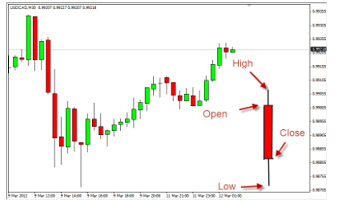
\includegraphics[scale=0.75]{imagenes/candleChart.png}
	\caption{Gráfico de vela.}
\end{figure}

La idea que vamos a adoptar para representar los estados, consiste en tomar esta idea de time frame y plasmarlos en la representación de los estados que se va a recibir el agente, es decir, el agente será capaz de ver una ventana de tiempo de tamaño n hacia atrás.

Teniendo en cuenta esto, vamos a definir a cada estado $S_t$  de la siguiente forma:

